%\documentclass[panstarrs,psreport,12pt]{panstarrs}
\documentclass[panstarrs]{panstarrs}
\usepackage{appendix}

% basic document variables
\title{Pan-STARRS MOPS Alert Concepts}
\subtitle{architecture for generating and distributing moving object alerts}
\author{Denver Green}
\shorttitle{Alerts}
\group{Pan-STARRS MOPS Group}
\project{Pan-STARRS Moving Objects Processing System}
\organization{Institute for Astronomy}
% \distribution{}
\version{02}
\docnumber{PSDC-530-006}
% note the use of the docnumber & version number:
% the complete PSDC document number is given by
% \thedocnumber-\theversion

\begin{document}
\maketitle

% -- Revision History --
\RevisionsStart
% version   Date         Description
02        & 2007.09.11 & Second draft \\
\hline
% 02        & 2003.03.05 & Second draft \\
\RevisionsEnd

% -- TBD / TBR Listing --
\TBDsStart
% section % page Date        Description
% 1.2.3.4   & 2    & xxx-xxx & missing a dingle on a dangle \\
\TBDsEnd

\pagebreak
\tableofcontents

\pagebreak
\listoffigures

\pagebreak 
\pagenumbering{arabic}
\section{Scope}
\subsection{Identification}
This document describes a system for the generation and distribution of moving 
object alerts. This system is developed as part of the Pan-STARRS Moving Object 
Processing System (MOPS).

\subsection{System Overview}
MOPS is the Pan-STARRS subsystem dedicated to discovering
asteroids and comets in Pan-STARRS detection catalogs.

\subsection{Document Overview}
MOPS generates new orbits for thousands of solar system objects. MOPS also refines known orbits when extra observations are associated to them. Some of these solar system objects prove to be of interest to a wider community. This might be because, for instance, of a high impact probability or a need to perform follow-up observations.

It is the responsibility of the Alert subsystem to determine if an object found by MOPS is `interesting` (in the sense given above). Once an object is determined to be interesting the Alert subsystem will generate an alert for that object. Interested parties within the community can then be notified of the alert and decide whether to act on it. In general, the MOPS Alert System is not a real-time system and a (small) lag between orbit publication in the MOPS database and alert publication is accepted.

The present document describes the architecture of the MOPS Alert System. 

\section{Architecture}
The MOPS Alert System is composed of four components
\begin{itemize}
\item MOPS Alert Generation (AlertUpdate, AlertCheck)
\item MOPS Alert Database
\item MOPS Alert Distribution (AlertSubmit)
\item MOPS Alert Clients (Twitter, Email, RSS) 
\end{itemize}

None of these components need to be co-located. In other words, the system is fully distributed and each component could (but does not need to) reside on a separate machine. See Figure 1 for a schematic representation of the four components that make up the MOPS Alert System. 

\begin{figure}
\begin{center}
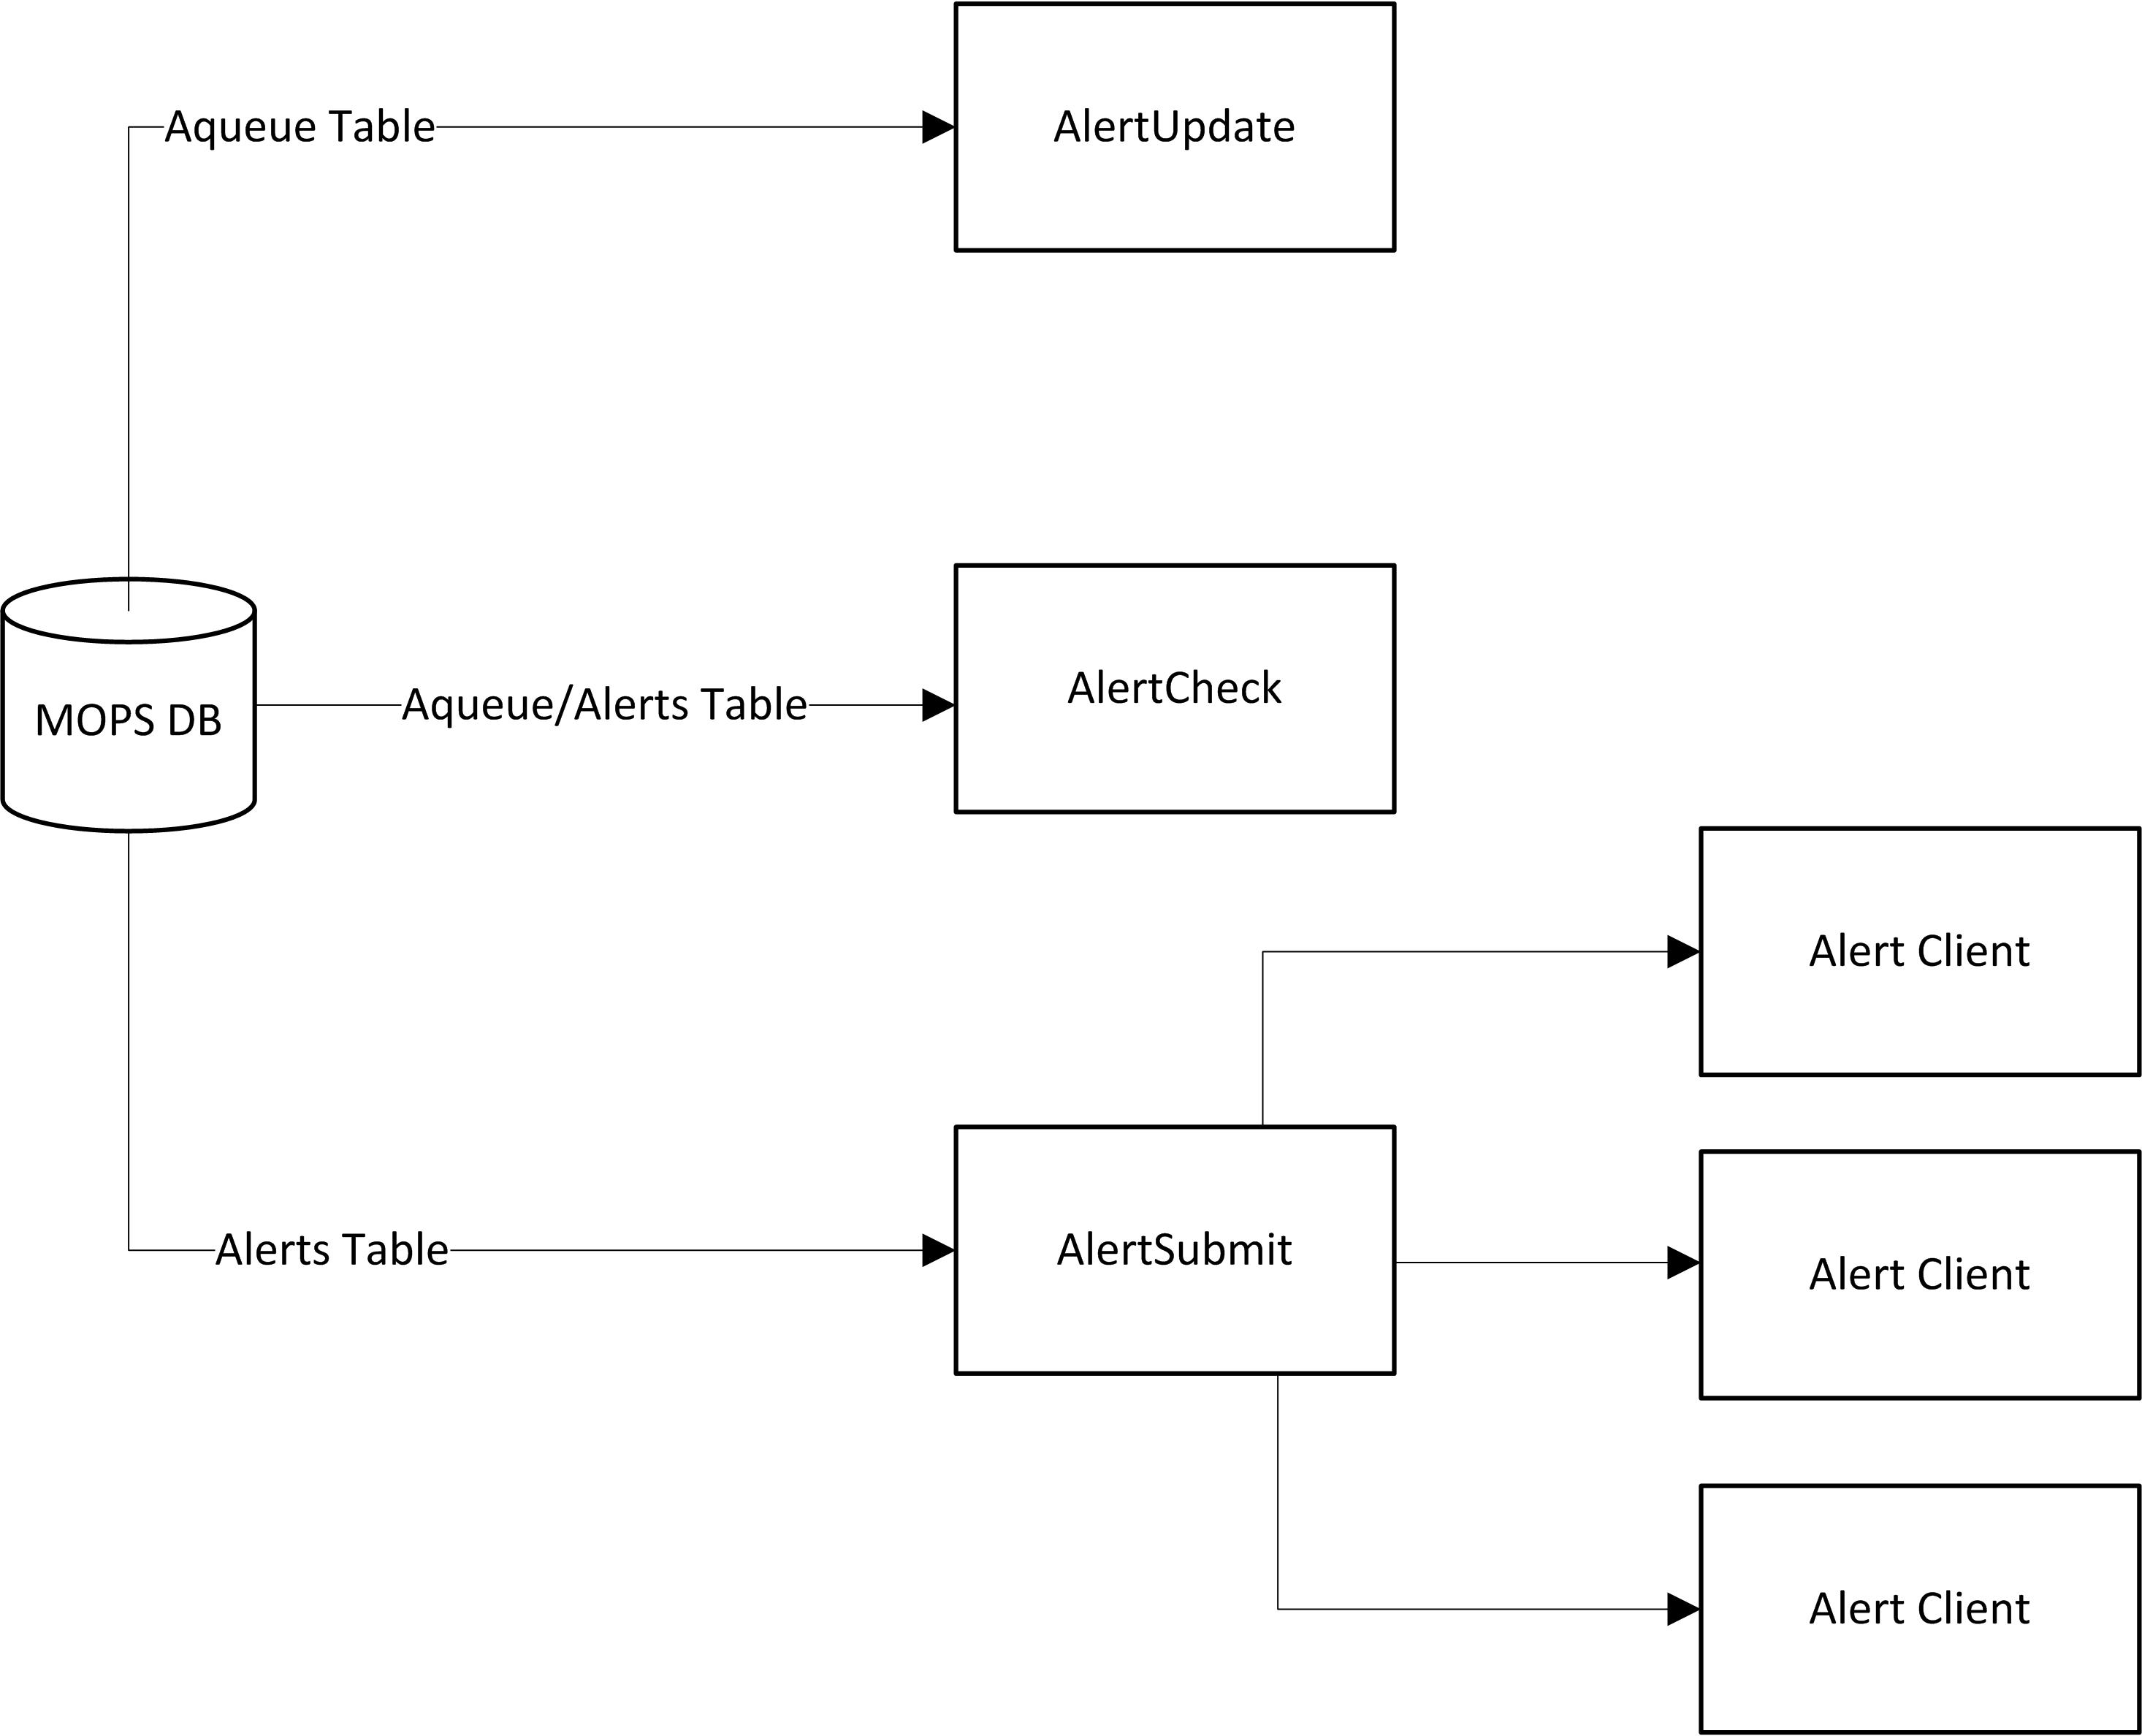
\includegraphics[width=7in]{AlertsArchitecture.jpg}
\caption{Architecture of the MOPS Alert Generation and Distribution System.}
\label{fig:architecture}
\end{center}
\end{figure}

\subsection{Alert Database}
The alert database consists of two tables (aqueue and alerts), and a view (v\_alerts) which is a join of the two tables. These tables are stored in a schema separate from the database schema that stores the MOPS data. This is done to allow the alert system to generate alerts for multiple MOPS schemas.

The aqueue table contains a reference to ALL tracklets and derived objects found by the alertupdate.py program. The aqueue table is the repository of all objects that potentially could be the subject of an alert. If a tracklet or derived object is not in the aqueue table then is cannot be the subject of an alert.

The status field in the aqueue table indicates if the object is new, available for processing, or has been processed.

The alerts table contains all derived objects and tracklets that have met the criteria of at least one alert rule executed by the alertcheck.py program. All alerts that are sent out by the alert system must come from this table. 

\begin{figure}
\begin{center}
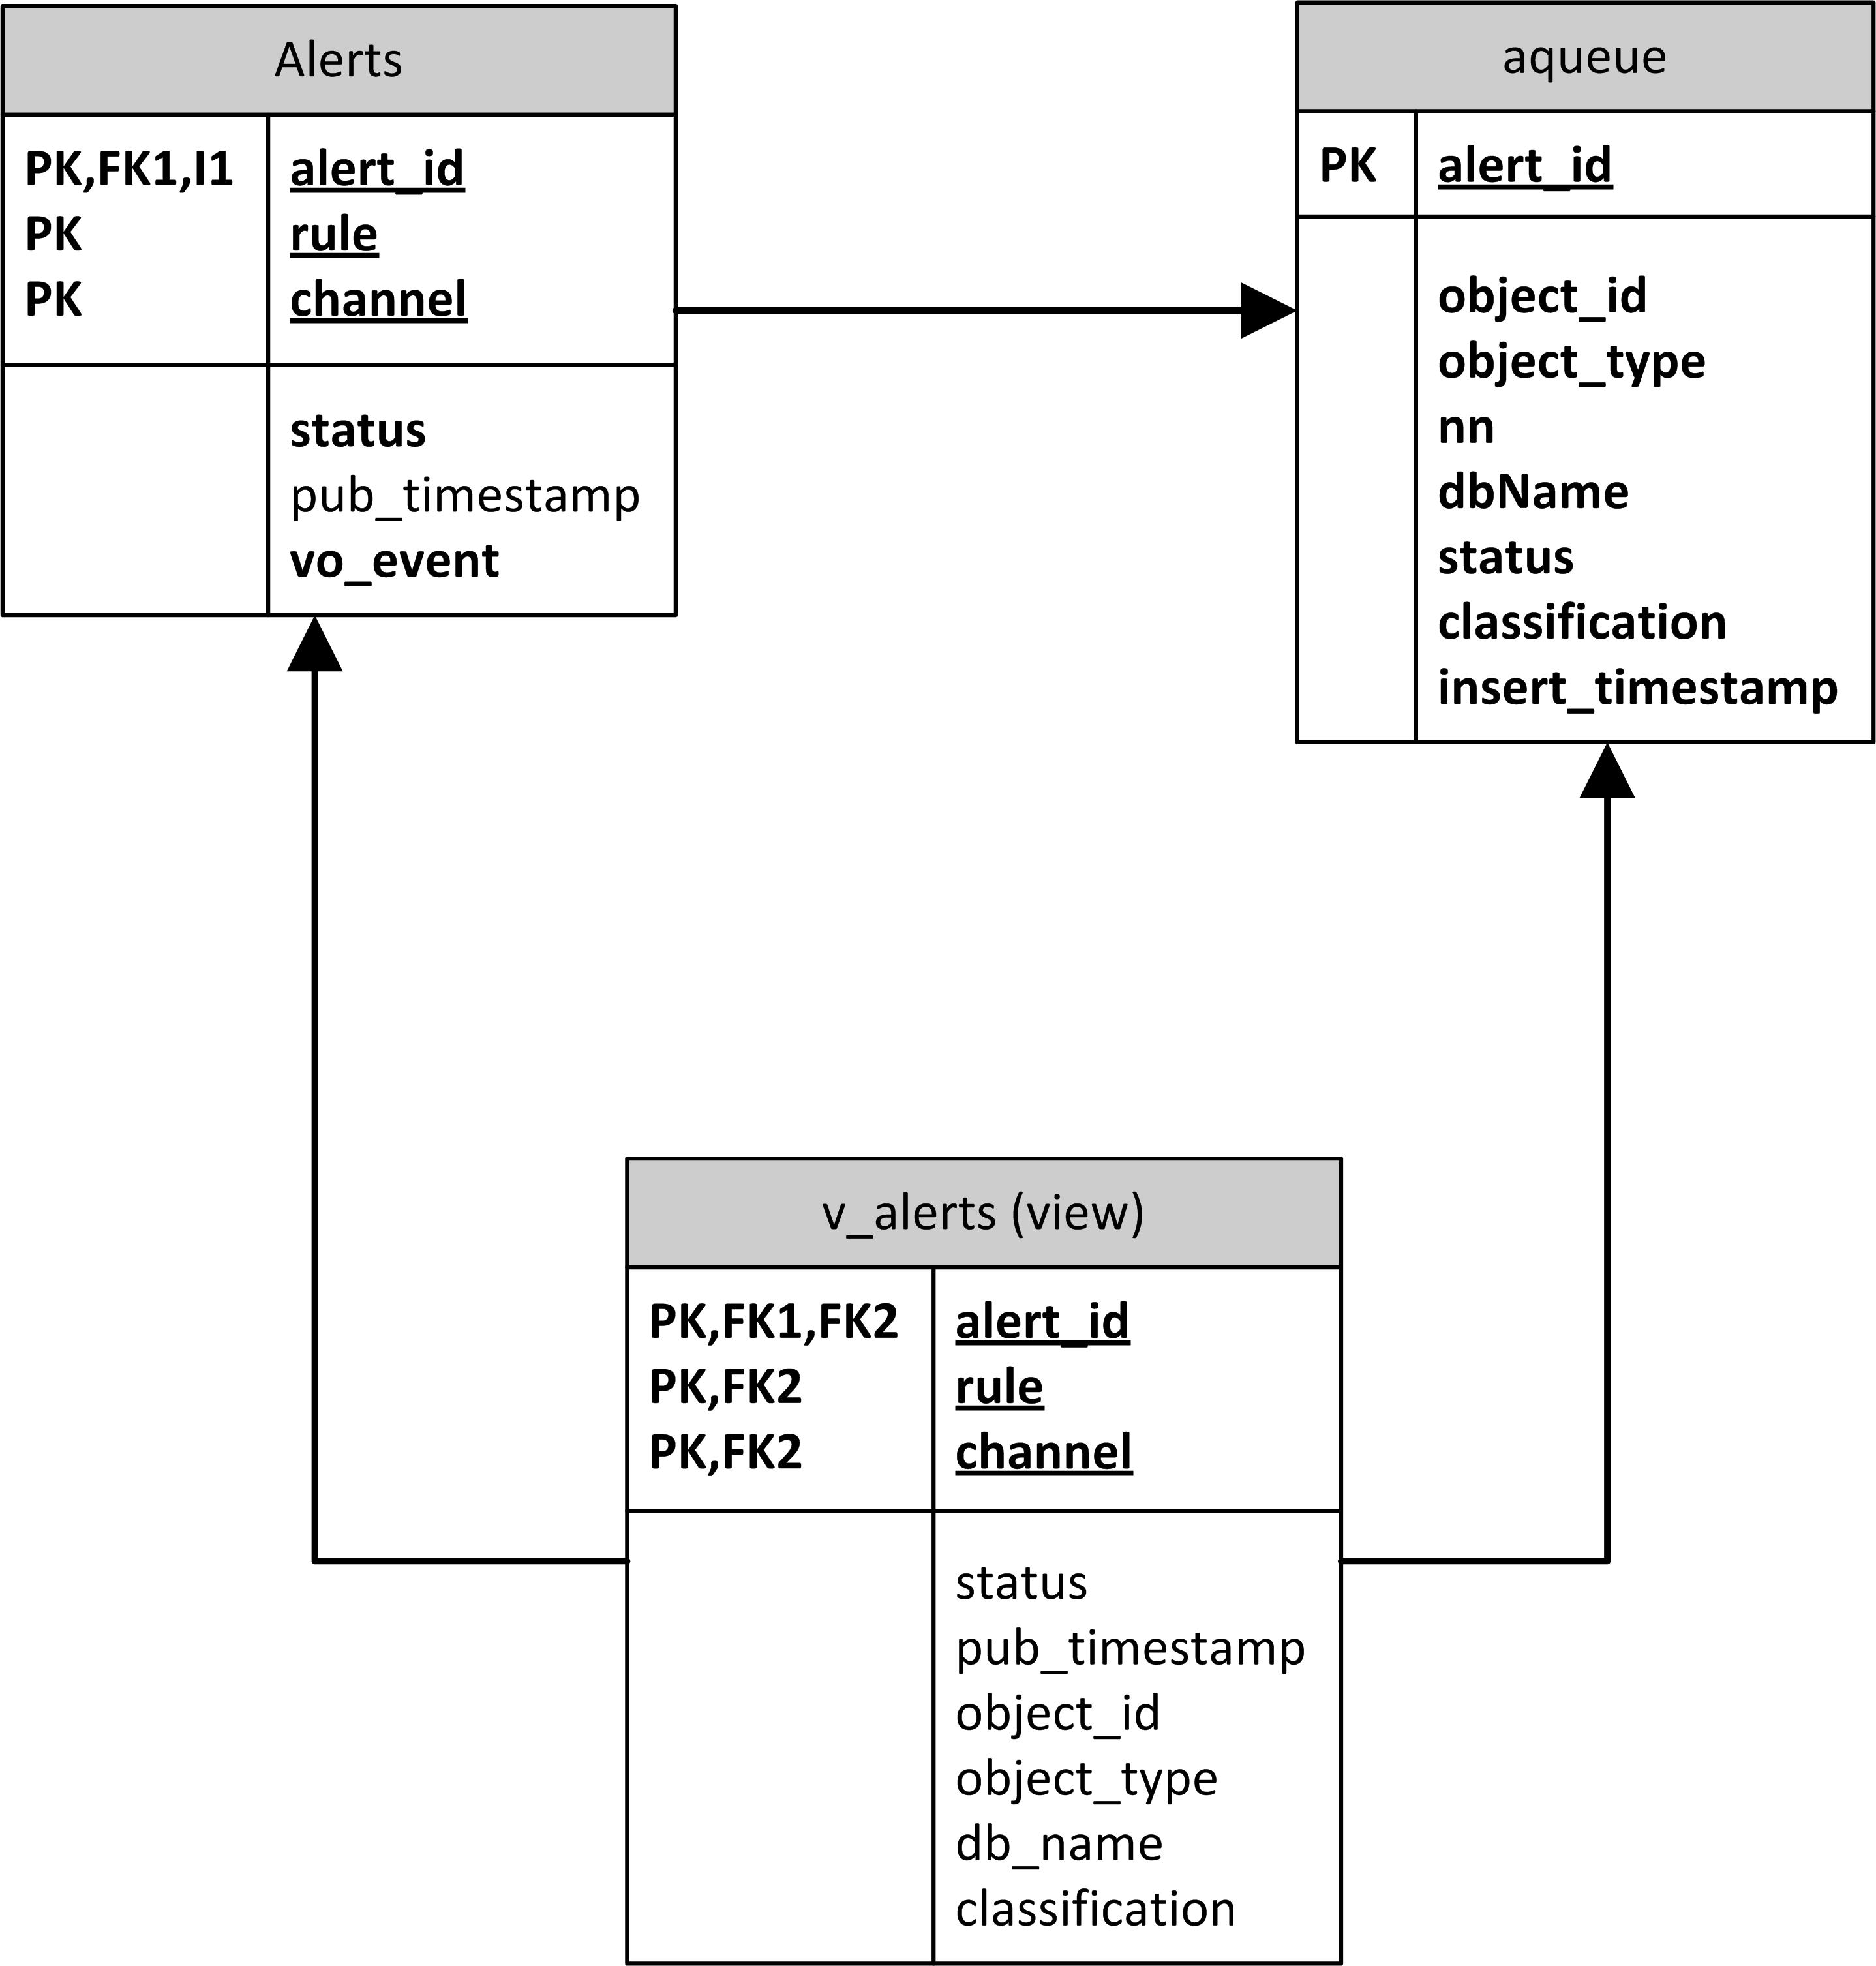
\includegraphics[width=7in]{Alerts_DB.jpg}
\caption{Database tables used by the Alert System}
\label{fig:database}
\end{center}
\end{figure}

\subsection{Alert Generation}
MOPS Alert Generation is done by two pieces of software (alertupdate and alertcheck) which determine which derived objects/tracklets to alert on.

The alertupdate program is responsible for extracting all of the derived objects/tracklets from a MOPS simulation that were created or modified after processing a night of observations. The objects found by alertupdate are written to the aqueue table in the alert database. The alertcheck program executes a set of rules (via a plugin architecture) against the data stored in the aqueue table. These rules identify which objects stored in the aqueue table need to be alerted on and for each object a entry is created in the alerts table.

The alertupdate program is invoked whenever mops fully completes the processing of a set of ingested exposures. Upon invocation, alertupdate will record information about all new and newly modified derived objects/tracklets in the simulation in the alert database, and mark it as new information ready for processing. The alertcheck program is then invoked and it will feed all new or modified derived objects/tracklets through all the rules registered with the alert system. Alertcheck will create an alert for all the derived objects/tracklets for which one or more alert rules evaluate to true. This alert will be stored in the alerts table. 

Alerts are generated on a per Derived Object/Tracklet basis (i.e. one alert per Derived Object and one Derived Object per alert). Alerts contain
\begin{itemize}
\item The orbital parameters for the Derived Object/Tracklet (i.e. q, e, i, node, time of perihelion passage, argument of the perihelion).
\item The epoch of the orbit.
\item The square root covariance matrix.
\item The residuals of the orbit determination.
\item The list of detections that were used to fit the orbit (with RA, Dec, epoch, filter and magnitude).
\item Geocentric ephemeris (with rate of motion, positional uncertainties and predicted magnitude) provided at 0h UT on a daily basis for 10 days starting on the date of the alert.
\item The name of the rule/rules that produced the alert.
\end{itemize}
Alerts are produced by alertcheck and are published by alertsubmit.


\subsubsection{Alert Rules}
Alert rules are user-supplied pieces of code that are implemented as Python modules imported by the alertcheck program. Each alert rule has access to the list of alert objects which is updated whenever MOPS processes a set of exposures. Each alert object contains a reference to a newly created or modified tracklet or derived object. Each rule exports one method called evaluate that has to return a list of Alert Objects that satisfy the rule. The structure of an Alert object is shown in figure 3. The most important attribute of the alert object is the alertObj attribute. This attribute points to a derived object if the rule subclasses the DerivedObjectRule or to a tracklet if the rule inherits from TrackletRule. A rule can examine the contents of a tracklet or derived object to see if they match the rule's criteria. For example the hyperbolics rule (see Appendix B) inherits from the DerivedbjectRule and returns a list of derived objects with an orbit that has a eccentricity (e) greater than 1, while the unlinked fast movers rule inherits from the TrackletRule and it returns a list of unattributed tracklets whose velocity is greater 0.99 degrees per day.

When writing a rule please keep in mind that you only have access to data associated with the tracklet or derived object that is being examined. Data from other tracklets or derivied objects is not accessible.

Figure 4 shows the database tables that underly the tracklet and derived object alert objects. These tables contain the attributes that you can use in your rules.

\begin{figure}
\begin{center}
\includegraphics[width=7in]{DerivedObject_Tracklet_DB_Schema.jpg}
\caption{ Alert object database tables}
\label{fig:do}
\end{center}
\end{figure}

\subsubsection{Alert Distribution}
Distribution of alerts is done by alertsubmit. The role of alertsubmit is to select all of the alerts in the alerts table which have not yet been published, and publish them. Alert distribution follows a publish-subscribe model.

When defining a rule a user can specify on which channel the rule should be published. A channel is just a way to select which twitter account, mail list, or RSS feed will be used to publish an alert. This allows subscribers to the alert system to select which category of alerts they want to be kept abreast of. Alertsubmit will automatically publish alerts to the all channel as well as to the channel specified in the rule.

The currently available channels are:
\begin{itemize}
\item all
\item centaurs
\item comets
\item hildas
\item hyperbolics
\item impactors
\item light
\item planets
\item sednas 
\end{itemize}



\subsubsection{Client}
Currently alerts are only published using twitter. To get an alert a user must have a twitter account which follows one or more of the following MOPS Twitter accounts.

\begin{itemize}
\item MopsAll
\item MopsCentaurs
\item MopsComets
\item MopsHildas
\item MopsHyperbolics
\item MopsImpactors
\item MopsLight
\item MopsPlanets
\item MopsSednas 
\end{itemize}

An alert sent via twitter will consist of a short text message which contains a link. Clicking on this link will download a XML file which represents a VOEvent. The VOEvent will contain the orbital data of the object that match the rule that triggered the alert.



\begin{appendices}
\section{Appendices}
\subsection{Example Alert Rule}
Alert Rules are written in Python and must inherit from MOPS.Alert.plugins.TrackletRule or MOPS.Alert.plugins.DerivedObjectRule. All rules inherit two instance variables (channel and alertObject) and five methods (evaluate, cleanup, newAlerts, getChannel, setChannel). Rules that inherit from DerivedObjectRule also inherit the instance variable minArcLength and the methods setMinArcLength and getMinArcLength :

\begin{figure}
\begin{center}
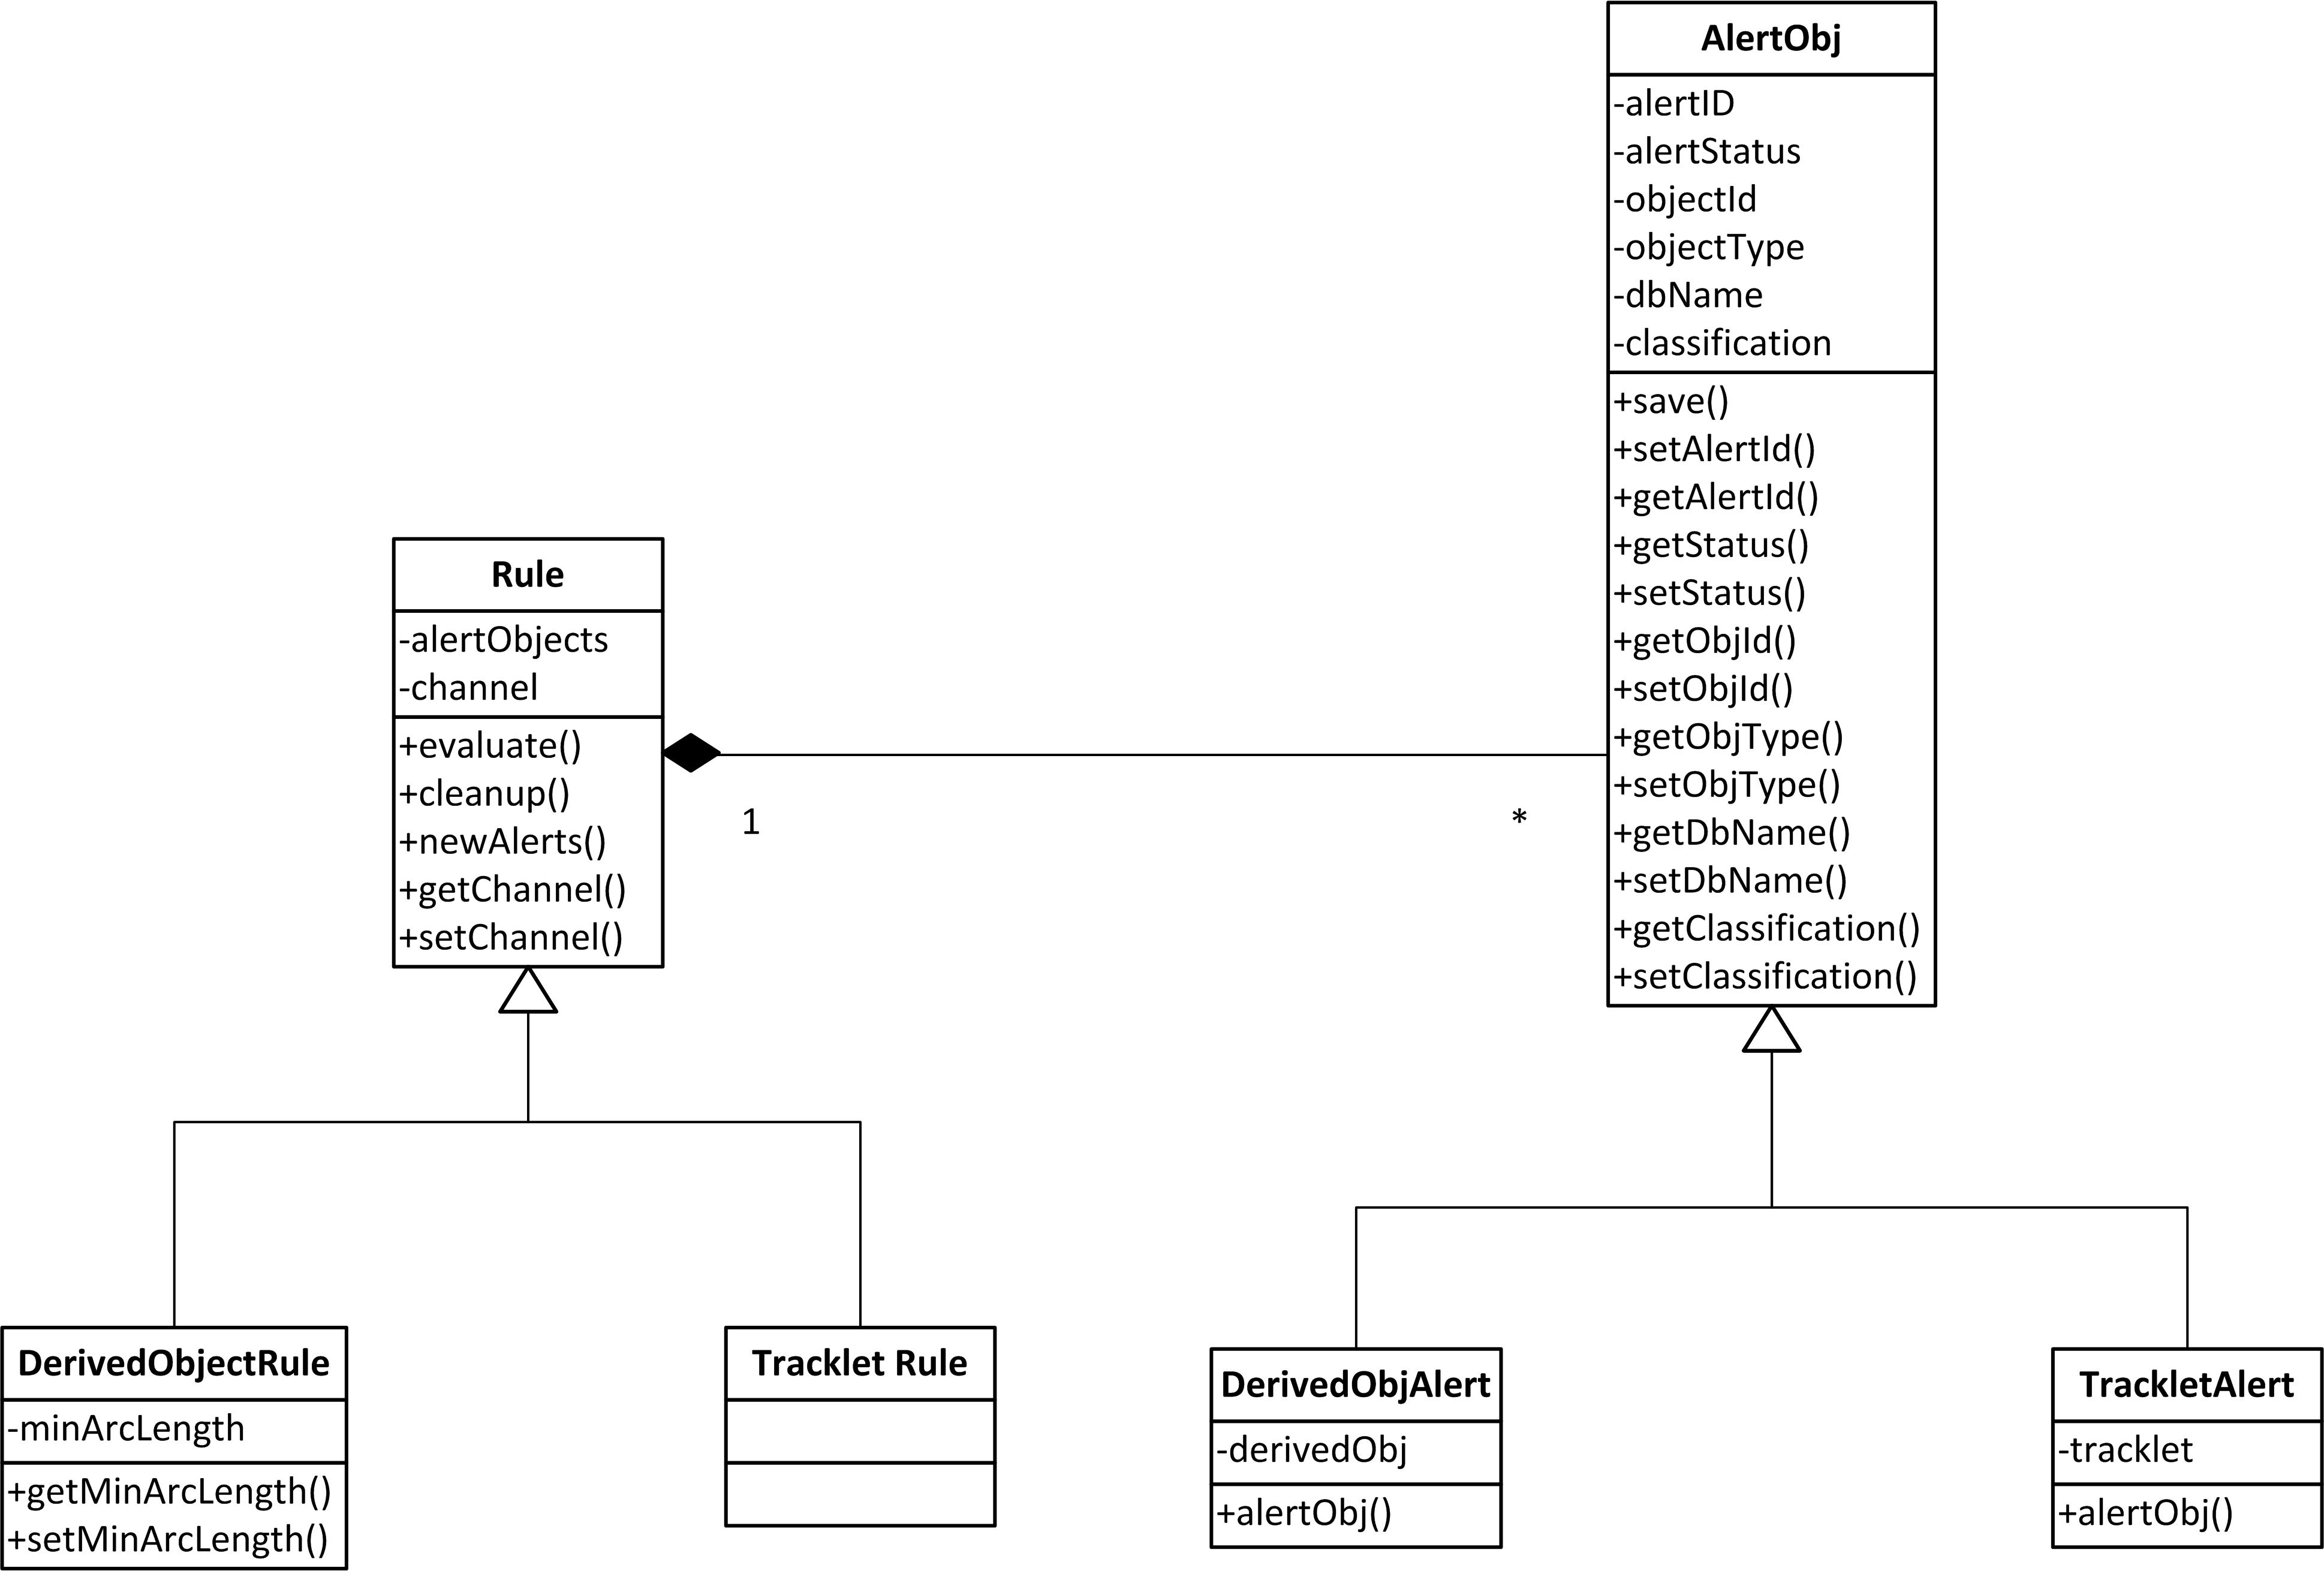
\includegraphics[width=7in]{Alerts.jpg}
\caption{ Alert System Class Diagram}
\label{fig:class}
\end{center}
\end{figure}

\begin{itemize}
\item channel: the name of the MOPS Alert channel that events generated by this rule are sent through. The currently available channels are:
\begin{itemize}
\item all
\item centaurs
\item comets
\item hildas
\item hyperbolics
\item impactors
\item light
\item planets
\item sednas 
\end{itemize}

\item alertObject: a list of newly created/modified DerivedObject and Tracklet instances. If a rule subclasses DerivedObjectRule then alertObject will contain a reference to a DerivedObject. If a rule subclasses TrackletRule then alertObject will contain a reference to a Tracklet. 

\item minArcLength: this applies only to rules that operate against derived objects and it specifies the minimum length of the orbital track the derived object must have in order to be considered by the rule. If minArcLength is not explicitly specified then it will default to zero. 
\end{itemize}

Alert Rules have to implement their own evaluate method since the default implementation raises a NotImplementedError exception. evaluate does not take any input and returns the list of AlertObject instances that satisfy the rule. In case no alert objects satisfy the rule, evaluate must return either the empty list or None. In case only one AlertObject is to be returned, evaluate must return the singleton list (i.e. a list composed of only one element) with that alert object as the only item. The cleanup method does not need to be implemented by a rule but is provided if there are resources used by the rule that need to be released after the execution of the rule.

What follows is an example Alert Rule that simply returns all newly created/modified AlertObjects which contain a reference to a DerivedObject.
\begin{verbatim}
class NewObjects(MOPS.Alert.plugins.DerivedObjectRule):
    """
    Return all new or newly modified DerivedObject instances.
    """
    def evaluate(self):
        """
        Return a list of AlertObject instances that satisfy the rule.
        """
        return(self.newAlerts())
\end{verbatim}

\subsection{Sample Alert Rules}
\subsubsection{Comets}
\begin{verbatim}
"""
plugins.comets

MOPS Alert Rule that returns DerivedObjects for which
   ( a>4.5 AU && e>0.5 ) || e>0.95
"""

from base import DerivedObjectRule
import sys
from MOPS.Alerts.plugins.Constants import CH_COMETS

class Comets(DerivedObjectRule):
   """
   Return all new or newly modified DerivedObject instances.
   """
   def IsComet(self, obj):
       """
       Return True if obj has ( a>4.5 AU && e>0.5 ) || e>0.95

       q = a * ( 1 - e )

       @param obj: DerivedObject instance
       """
       return(obj.alertObj.orbit.e > 0.95 or
              (obj.alertObj.orbit.e > 0.5 and obj.alertObj.orbit.q / (1 - obj.alertObj.orbit.e) > 4.5))

   
   def evaluate(self):
       """
       Return a list of DerivedObject instances that satisfy the rule.
       """
       
       #Set the channel that will be used to publish the alert.
       self.channel = CH_COMETS
       return([obj for obj in self.newAlerts if self.IsComet(obj)])
# <-- end class
\end{verbatim}

\subsubsection{Distant Planets}
\begin{verbatim}
"""
plugins.distant_planets

MOPS Alert Rule that returns DerivedObjects for which
   a > 60 AU
"""

from base import DerivedObjectRule
from MOPS.Alerts.plugins.Constants import CH_PLANETS
import sys

class DistantPlanets(DerivedObjectRule):
   """
   Return all new or newly modified DerivedObject instances.
   """
   def isDistantPlanet(self, obj):
       """
       Return True if obj has a > 60 AU

       q = a * ( 1 - e )

       @param obj: DerivedObject instance
       """
       return(obj.alertObj.orbit.q / (1 - obj.alertObj.orbit.e) > 60)

   
   def evaluate(self):
       """
       Return a list of DerivedObject instances that satisfy the rule.
       """
       #Set the channel that will be used to publish the alert.
       self.channel = CH_PLANETS
       return([obj for obj in self.newAlerts \
               if self.isDistantPlanet(obj)])
# <-- end class
\end{verbatim}

\subsubsection{Hyperbolics}
\begin{verbatim}
"""
plugins.hyperbolics

MOPS Alert Rule that returns DerivedObjects for which
   e > 1.0
"""

from base import DerivedObjectRule
from MOPS.Alerts.plugins.Constants import CH_HYPERBOLICS
import sys

class Hyperbolics(DerivedObjectRule):
   """
   Return all new or newly modified DerivedObject instances.
   """
   def isHyperbolic(self, obj):
       """
       Return True if obj has e > 1.0

       @param obj: DerivedObject instance
       """
       return(obj.alertObj.orbit.e > 1.0)
 
   def evaluate(self):
       """
       Return a list of DerivedObject instances that satisfy the rule.
       """
       #Set the channel that will be used to publish the alert.
       self.channel = CH_HYPERBOLICS
       return([obj for obj in self.newAlerts \
               if self.isHyperbolic(obj)])
# <-- end class
\end{verbatim}

\subsubsection{Impactors}
\begin{verbatim}
"""
plugins.impactors

MOPS Alert Rule that returns DerivedObjects for which
   moid_1<0.005 AU OR moid_2<0.005 AU
"""

from base import DerivedObjectRule
from MOPS.Alerts.plugins.Constants import CH_IMPACTORS
import sys

class Impactors(DerivedObjectRule):
   """
   Return all new or newly modified DerivedObject instances.
   """
   def isImpactor(self, obj):
       """
       Return True if obj has moid_1<0.005 AU OR moid_2<0.005 AU

       @param obj: DerivedObject instance
       """
       return((obj.alertObj.orbit.moid_1 != None and obj.alertObj.orbit.moid_1 < 0.005) or
              ((obj.alertObj.orbit.moid_2 != None and obj.alertObj.orbit.moid_2 < 0.005)))
   
   def evaluate(self):
       """
       Return a list of DerivedObject instances that satisfy the rule.
       """
       #Set the channel that will be used to publish the alert.
       self.channel = CH_IMPACTORS
       return([obj for obj in self.newAlerts if self.isImpactor(obj)])
# <-- end class
\end{verbatim}

\subsubsection{Unusual Light Curves}
\begin{verbatim}
"""
plugins.unusual_light_curve

MOPS Alert Rule that returns DerivedObjects for which either one is true:
   1. the difference in magnitude between detections in any given tracklet
      is > 0.3 mag.
   2. the min-max magnitude amongst all detections is > 1.0 mag.
"""

from base import DerivedObjectRule
from MOPS.Alerts.plugins.Constants import CH_LIGHT
import sys

class UnusualLightCurves(DerivedObjectRule):
   """
   Return all new or newly modified DerivedObject instances.
   """
   def isUnusual(self, obj):
       """
       Return True if either one is true for obj:
       1. the difference in magnitude between detections in any given tracklet
          is > 0.3 mag.
       2. the min-max magnitude amongst all detections is > 1.0 mag.

       @param obj: DerivedObject instance
       """
       tracklets = obj.alertObj.tracklets

       # First, check rule number 1.
       allMags = []
       for t in tracklets:
           mags = [d.mag for d in t.detections]
           mags.sort()
           if(abs(mags[-1] - mags[0]) > 0.3):
               return(True)
           # <-- end if

           # That was not True, update allMags just in case we have to test
           # rule 2 as well.
           allMags += mags
       # <-- end for
       
       # Then rule number 2.
       allMags.sort()
       return(abs(allMags[-1] - allMags[0]) > 1.)
   
   def evaluate(self):
       """
       Return a list of DerivedObject instances that satisfy the rule.
       """
       #Set the channel that will be used to publish the alert.
       self.channel = CH_LIGHT
       return([obj for obj in self.newAlerts if self.isUnusual(obj)])
# <-- end class
\end{verbatim}

\subsubsection{Unlinked Fast Movers}
\begin{verbatim}
"""
plugins.unlinked_fast_movers

MOPS Alert Rule that returns Tracklets which
   1. Are unlinked
   2. Have velocity > 0.5 deg/day
"""

from MOPS.Tracklet import Tracklet
from MOPS.Constants import TRACKLET_STATUS_UNATTRIBUTED
from base import TrackletRule

# Constants
MIN_VELOCITY = 0.99      # Minimum velocity a tracklet must have.            

class UnlinkedFastMovers(TrackletRule):
   def isFastMover(self, tracklet):
       """
       Return True if the tracklet has a velocity > MIN_VELOCITY deg/day

       @param obj: tracklet to be tested.
       @rtype: boolean
       """
       return(tracklet.vTot > MIN_VELOCITY)
   # <-- end is FastMover
   
   def evaluate(self):
       """
       Return a list of Tracklet instances that satisfy the rule.

       Return all unattributed Tracklets which have a velocity > MIN_VELOCITY 
       deg/day.
       """
       alerts = []

       # Get tracklets that are ready for processing.
       for obj in self.newAlerts:
           if (obj.alertObj.status == TRACKLET_STATUS_UNATTRIBUTED):
               # Process only unattributed tracklets.
               if (self.isFastMover(obj.alertObj)):
                   alerts.append(obj)
               # <-- end if
           # <-- end if
       # <-- end for
       return(alerts)
   # <-- end evaluate
# <-- end UnlinkedFastMovers
\end{verbatim}


\subsection{Sample VOEvent}
VOEvent is a way to represent astronomical events using XML. The MOPS alerts system uses this standard to reresent alerts. For more information about VOEvents you can read the Wikipedia entry for it at http://en.wikipedia.org/wiki/VOEvent.

Below is a sample VOEvent generated by MOPS.
\begin{verbatim}
<?xml version="1.0" encoding="utf-8"?>
<VOEvent ivorn="ivo://mops.lsst.org/VOEvent#psmops_ps1_mdrm137_7447_2011-08-04T20:16:36.47_" role="observation" version="1.1" xmlns="http://www.ivoa.net/xml/VOEvent/v1.1">
           <!-- This document was generated by MOPS -->
  <Who>
    <AuthorIVORN>ivo://voevent.lsst.org/MOPS</AuthorIVORN>
    <Date>2011-08-04T20:16:36.47</Date>
  </Who>
  <WhereWhen>
    <!-- Detections -->
    <ObsDataLocation description="Observations" xmlns="http://www.ivoa.net/xml/STC/stc-v1.30.xsd">
      <ObservatoryLocation id="MOPS" type="simple" href="ivo://STClib/Observatories#MOPS"/>
      <ObservationLocation>
        <AstroCoords coord_system_id="UTC-ICRS-TOPO-VMAG">
          <ScalarCoordinate unit="mag" frame_id="Vmag">
            <Value>18.35</Value>
          </ScalarCoordinate>
          <Time>
            <TimeInstant>
              <MJDTime>55678.448951</MJDTime>
            </TimeInstant>
          </Time>
          <Position2D unit="deg">
            <Value2>
              <C1>231.769276</C1>
              <C2>-3.793327</C2>
            </Value2>
          </Position2D>
        </AstroCoords>
      </ObservationLocation>
    </ObsDataLocation>
    <ObsDataLocation description="Observations" xmlns="http://www.ivoa.net/xml/STC/stc-v1.30.xsd">
      <ObservatoryLocation id="MOPS" type="simple" href="ivo://STClib/Observatories#MOPS"/>
      <ObservationLocation>
        <AstroCoords coord_system_id="UTC-ICRS-TOPO-VMAG">
          <ScalarCoordinate unit="mag" frame_id="Vmag">
            <Value>18.32</Value>
          </ScalarCoordinate>
          <Time>
            <TimeInstant>
              <MJDTime>55678.458742</MJDTime>
            </TimeInstant>
          </Time>
          <Position2D unit="deg">
            <Value2>
              <C1>231.766977</C1>
              <C2>-3.793560</C2>
            </Value2>
          </Position2D>
        </AstroCoords>
      </ObservationLocation>
    </ObsDataLocation>
    <ObsDataLocation description="Observations" xmlns="http://www.ivoa.net/xml/STC/stc-v1.30.xsd">
      <ObservatoryLocation id="MOPS" type="simple" href="ivo://STClib/Observatories#MOPS"/>
      <ObservationLocation>
        <AstroCoords coord_system_id="UTC-ICRS-TOPO-VMAG">
          <ScalarCoordinate unit="mag" frame_id="Vmag">
            <Value>17.87</Value>
          </ScalarCoordinate>
          <Time>
            <TimeInstant>
              <MJDTime>55678.470619</MJDTime>
            </TimeInstant>
          </Time>
          <Position2D unit="deg">
            <Value2>
              <C1>231.764195</C1>
              <C2>-3.793831</C2>
            </Value2>
          </Position2D>
        </AstroCoords>
      </ObservationLocation>
    </ObsDataLocation>
    <ObsDataLocation description="Observations" xmlns="http://www.ivoa.net/xml/STC/stc-v1.30.xsd">
      <ObservatoryLocation id="MOPS" type="simple" href="ivo://STClib/Observatories#MOPS"/>
      <ObservationLocation>
        <AstroCoords coord_system_id="UTC-ICRS-TOPO-VMAG">
          <ScalarCoordinate unit="mag" frame_id="Vmag">
            <Value>17.82</Value>
          </ScalarCoordinate>
          <Time>
            <TimeInstant>
              <MJDTime>55678.481330</MJDTime>
            </TimeInstant>
          </Time>
          <Position2D unit="deg">
            <Value2>
              <C1>231.761692</C1>
              <C2>-3.794059</C2>
            </Value2>
          </Position2D>
        </AstroCoords>
      </ObservationLocation>
    </ObsDataLocation>
    <ObsDataLocation description="Observations" xmlns="http://www.ivoa.net/xml/STC/stc-v1.30.xsd">
      <ObservatoryLocation id="MOPS" type="simple" href="ivo://STClib/Observatories#MOPS"/>
      <ObservationLocation>
        <AstroCoords coord_system_id="UTC-ICRS-TOPO-VMAG">
          <ScalarCoordinate unit="mag" frame_id="Vmag">
            <Value>18.20</Value>
          </ScalarCoordinate>
          <Time>
            <TimeInstant>
              <MJDTime>55679.401333</MJDTime>
            </TimeInstant>
          </Time>
          <Position2D unit="deg">
            <Value2>
              <C1>231.552585</C1>
              <C2>-3.815721</C2>
            </Value2>
          </Position2D>
        </AstroCoords>
      </ObservationLocation>
    </ObsDataLocation>
    <ObsDataLocation description="Observations" xmlns="http://www.ivoa.net/xml/STC/stc-v1.30.xsd">
      <ObservatoryLocation id="MOPS" type="simple" href="ivo://STClib/Observatories#MOPS"/>
      <ObservationLocation>
        <AstroCoords coord_system_id="UTC-ICRS-TOPO-VMAG">
          <ScalarCoordinate unit="mag" frame_id="Vmag">
            <Value>18.27</Value>
          </ScalarCoordinate>
          <Time>
            <TimeInstant>
              <MJDTime>55679.416640</MJDTime>
            </TimeInstant>
          </Time>
          <Position2D unit="deg">
            <Value2>
              <C1>231.548945</C1>
              <C2>-3.816108</C2>
            </Value2>
          </Position2D>
        </AstroCoords>
      </ObservationLocation>
    </ObsDataLocation>
    <ObsDataLocation description="Observations" xmlns="http://www.ivoa.net/xml/STC/stc-v1.30.xsd">
      <ObservatoryLocation id="MOPS" type="simple" href="ivo://STClib/Observatories#MOPS"/>
      <ObservationLocation>
        <AstroCoords coord_system_id="UTC-ICRS-TOPO-VMAG">
          <ScalarCoordinate unit="mag" frame_id="Vmag">
            <Value>17.65</Value>
          </ScalarCoordinate>
          <Time>
            <TimeInstant>
              <MJDTime>55679.432748</MJDTime>
            </TimeInstant>
          </Time>
          <Position2D unit="deg">
            <Value2>
              <C1>231.545099</C1>
              <C2>-3.816500</C2>
            </Value2>
          </Position2D>
        </AstroCoords>
      </ObservationLocation>
    </ObsDataLocation>
    <ObsDataLocation description="Observations" xmlns="http://www.ivoa.net/xml/STC/stc-v1.30.xsd">
      <ObservatoryLocation id="MOPS" type="simple" href="ivo://STClib/Observatories#MOPS"/>
      <ObservationLocation>
        <AstroCoords coord_system_id="UTC-ICRS-TOPO-VMAG">
          <ScalarCoordinate unit="mag" frame_id="Vmag">
            <Value>17.63</Value>
          </ScalarCoordinate>
          <Time>
            <TimeInstant>
              <MJDTime>55679.447325</MJDTime>
            </TimeInstant>
          </Time>
          <Position2D unit="deg">
            <Value2>
              <C1>231.541619</C1>
              <C2>-3.816865</C2>
            </Value2>
          </Position2D>
        </AstroCoords>
      </ObservationLocation>
    </ObsDataLocation>
    <ObsDataLocation description="Observations" xmlns="http://www.ivoa.net/xml/STC/stc-v1.30.xsd">
      <ObservatoryLocation id="MOPS" type="simple" href="ivo://STClib/Observatories#MOPS"/>
      <ObservationLocation>
        <AstroCoords coord_system_id="UTC-ICRS-TOPO-VMAG">
          <ScalarCoordinate unit="mag" frame_id="Vmag">
            <Value>17.81</Value>
          </ScalarCoordinate>
          <Time>
            <TimeInstant>
              <MJDTime>55682.425996</MJDTime>
            </TimeInstant>
          </Time>
          <Position2D unit="deg">
            <Value2>
              <C1>230.839751</C1>
              <C2>-3.898394</C2>
            </Value2>
          </Position2D>
        </AstroCoords>
      </ObservationLocation>
    </ObsDataLocation>
    <ObsDataLocation description="Observations" xmlns="http://www.ivoa.net/xml/STC/stc-v1.30.xsd">
      <ObservatoryLocation id="MOPS" type="simple" href="ivo://STClib/Observatories#MOPS"/>
      <ObservationLocation>
        <AstroCoords coord_system_id="UTC-ICRS-TOPO-VMAG">
          <ScalarCoordinate unit="mag" frame_id="Vmag">
            <Value>17.77</Value>
          </ScalarCoordinate>
          <Time>
            <TimeInstant>
              <MJDTime>55682.440097</MJDTime>
            </TimeInstant>
          </Time>
          <Position2D unit="deg">
            <Value2>
              <C1>230.836234</C1>
              <C2>-3.898824</C2>
            </Value2>
          </Position2D>
        </AstroCoords>
      </ObservationLocation>
    </ObsDataLocation>
    <ObsDataLocation description="Observations" xmlns="http://www.ivoa.net/xml/STC/stc-v1.30.xsd">
      <ObservatoryLocation id="MOPS" type="simple" href="ivo://STClib/Observatories#MOPS"/>
      <ObservationLocation>
        <AstroCoords coord_system_id="UTC-ICRS-TOPO-VMAG">
          <ScalarCoordinate unit="mag" frame_id="Vmag">
            <Value>17.80</Value>
          </ScalarCoordinate>
          <Time>
            <TimeInstant>
              <MJDTime>55682.454299</MJDTime>
            </TimeInstant>
          </Time>
          <Position2D unit="deg">
            <Value2>
              <C1>230.832679</C1>
              <C2>-3.899250</C2>
            </Value2>
          </Position2D>
        </AstroCoords>
      </ObservationLocation>
    </ObsDataLocation>
    <ObsDataLocation description="Observations" xmlns="http://www.ivoa.net/xml/STC/stc-v1.30.xsd">
      <ObservatoryLocation id="MOPS" type="simple" href="ivo://STClib/Observatories#MOPS"/>
      <ObservationLocation>
        <AstroCoords coord_system_id="UTC-ICRS-TOPO-VMAG">
          <ScalarCoordinate unit="mag" frame_id="Vmag">
            <Value>17.78</Value>
          </ScalarCoordinate>
          <Time>
            <TimeInstant>
              <MJDTime>55682.468390</MJDTime>
            </TimeInstant>
          </Time>
          <Position2D unit="deg">
            <Value2>
              <C1>230.829160</C1>
              <C2>-3.899678</C2>
            </Value2>
          </Position2D>
        </AstroCoords>
      </ObservationLocation>
    </ObsDataLocation>
    <ObsDataLocation description="Observations" xmlns="http://www.ivoa.net/xml/STC/stc-v1.30.xsd">
      <ObservatoryLocation id="MOPS" type="simple" href="ivo://STClib/Observatories#MOPS"/>
      <ObservationLocation>
        <AstroCoords coord_system_id="UTC-ICRS-TOPO-VMAG">
          <ScalarCoordinate unit="mag" frame_id="Vmag">
            <Value>18.15</Value>
          </ScalarCoordinate>
          <Time>
            <TimeInstant>
              <MJDTime>55692.520542</MJDTime>
            </TimeInstant>
          </Time>
          <Position2D unit="deg">
            <Value2>
              <C1>228.289393</C1>
              <C2>-4.312864</C2>
            </Value2>
          </Position2D>
        </AstroCoords>
      </ObservationLocation>
    </ObsDataLocation>
    <ObsDataLocation description="Observations" xmlns="http://www.ivoa.net/xml/STC/stc-v1.30.xsd">
      <ObservatoryLocation id="MOPS" type="simple" href="ivo://STClib/Observatories#MOPS"/>
      <ObservationLocation>
        <AstroCoords coord_system_id="UTC-ICRS-TOPO-VMAG">
          <ScalarCoordinate unit="mag" frame_id="Vmag">
            <Value>18.19</Value>
          </ScalarCoordinate>
          <Time>
            <TimeInstant>
              <MJDTime>55692.530696</MJDTime>
            </TimeInstant>
          </Time>
          <Position2D unit="deg">
            <Value2>
              <C1>228.286673</C1>
              <C2>-4.313388</C2>
            </Value2>
          </Position2D>
        </AstroCoords>
      </ObservationLocation>
    </ObsDataLocation>
    <ObsDataLocation description="Observations" xmlns="http://www.ivoa.net/xml/STC/stc-v1.30.xsd">
      <ObservatoryLocation id="MOPS" type="simple" href="ivo://STClib/Observatories#MOPS"/>
      <ObservationLocation>
        <AstroCoords coord_system_id="UTC-ICRS-TOPO-VMAG">
          <ScalarCoordinate unit="mag" frame_id="Vmag">
            <Value>18.51</Value>
          </ScalarCoordinate>
          <Time>
            <TimeInstant>
              <MJDTime>55746.259619</MJDTime>
            </TimeInstant>
          </Time>
          <Position2D unit="deg">
            <Value2>
              <C1>219.778845</C1>
              <C2>-10.155196</C2>
            </Value2>
          </Position2D>
        </AstroCoords>
      </ObservationLocation>
    </ObsDataLocation>
    <ObsDataLocation description="Observations" xmlns="http://www.ivoa.net/xml/STC/stc-v1.30.xsd">
      <ObservatoryLocation id="MOPS" type="simple" href="ivo://STClib/Observatories#MOPS"/>
      <ObservationLocation>
        <AstroCoords coord_system_id="UTC-ICRS-TOPO-VMAG">
          <ScalarCoordinate unit="mag" frame_id="Vmag">
            <Value>18.32</Value>
          </ScalarCoordinate>
          <Time>
            <TimeInstant>
              <MJDTime>55746.274136</MJDTime>
            </TimeInstant>
          </Time>
          <Position2D unit="deg">
            <Value2>
              <C1>219.778844</C1>
              <C2>-10.157382</C2>
            </Value2>
          </Position2D>
        </AstroCoords>
      </ObservationLocation>
    </ObsDataLocation>
    <ObsDataLocation description="Observations" xmlns="http://www.ivoa.net/xml/STC/stc-v1.30.xsd">
      <ObservatoryLocation id="MOPS" type="simple" href="ivo://STClib/Observatories#MOPS"/>
      <ObservationLocation>
        <AstroCoords coord_system_id="UTC-ICRS-TOPO-VMAG">
          <ScalarCoordinate unit="mag" frame_id="Vmag">
            <Value>18.49</Value>
          </ScalarCoordinate>
          <Time>
            <TimeInstant>
              <MJDTime>55746.285891</MJDTime>
            </TimeInstant>
          </Time>
          <Position2D unit="deg">
            <Value2>
              <C1>219.778848</C1>
              <C2>-10.159156</C2>
            </Value2>
          </Position2D>
        </AstroCoords>
      </ObservationLocation>
    </ObsDataLocation>
    <ObsDataLocation description="Observations" xmlns="http://www.ivoa.net/xml/STC/stc-v1.30.xsd">
      <ObservatoryLocation id="MOPS" type="simple" href="ivo://STClib/Observatories#MOPS"/>
      <ObservationLocation>
        <AstroCoords coord_system_id="UTC-ICRS-TOPO-VMAG">
          <ScalarCoordinate unit="mag" frame_id="Vmag">
            <Value>18.45</Value>
          </ScalarCoordinate>
          <Time>
            <TimeInstant>
              <MJDTime>55746.296664</MJDTime>
            </TimeInstant>
          </Time>
          <Position2D unit="deg">
            <Value2>
              <C1>219.778833</C1>
              <C2>-10.160801</C2>
            </Value2>
          </Position2D>
        </AstroCoords>
      </ObservationLocation>
    </ObsDataLocation>
    <ObsDataLocation description="Observations" xmlns="http://www.ivoa.net/xml/STC/stc-v1.30.xsd">
      <ObservatoryLocation id="MOPS" type="simple" href="ivo://STClib/Observatories#MOPS"/>
      <ObservationLocation>
        <AstroCoords coord_system_id="UTC-ICRS-TOPO-VMAG">
          <ScalarCoordinate unit="mag" frame_id="Vmag">
            <Value>18.55</Value>
          </ScalarCoordinate>
          <Time>
            <TimeInstant>
              <MJDTime>55757.276107</MJDTime>
            </TimeInstant>
          </Time>
          <Position2D unit="deg">
            <Value2>
              <C1>220.267380</C1>
              <C2>-11.866986</C2>
            </Value2>
          </Position2D>
        </AstroCoords>
      </ObservationLocation>
    </ObsDataLocation>
    <ObsDataLocation description="Observations" xmlns="http://www.ivoa.net/xml/STC/stc-v1.30.xsd">
      <ObservatoryLocation id="MOPS" type="simple" href="ivo://STClib/Observatories#MOPS"/>
      <ObservationLocation>
        <AstroCoords coord_system_id="UTC-ICRS-TOPO-VMAG">
          <ScalarCoordinate unit="mag" frame_id="Vmag">
            <Value>18.57</Value>
          </ScalarCoordinate>
          <Time>
            <TimeInstant>
              <MJDTime>55757.287801</MJDTime>
            </TimeInstant>
          </Time>
          <Position2D unit="deg">
            <Value2>
              <C1>220.268243</C1>
              <C2>-11.868819</C2>
            </Value2>
          </Position2D>
        </AstroCoords>
      </ObservationLocation>
    </ObsDataLocation>
    <ObsDataLocation description="Observations" xmlns="http://www.ivoa.net/xml/STC/stc-v1.30.xsd">
      <ObservatoryLocation id="MOPS" type="simple" href="ivo://STClib/Observatories#MOPS"/>
      <ObservationLocation>
        <AstroCoords coord_system_id="UTC-ICRS-TOPO-VMAG">
          <ScalarCoordinate unit="mag" frame_id="Vmag">
            <Value>18.20</Value>
          </ScalarCoordinate>
          <Time>
            <TimeInstant>
              <MJDTime>55761.251771</MJDTime>
            </TimeInstant>
          </Time>
          <Position2D unit="deg">
            <Value2>
              <C1>220.635041</C1>
              <C2>-12.504146</C2>
            </Value2>
          </Position2D>
        </AstroCoords>
      </ObservationLocation>
    </ObsDataLocation>
    <ObsDataLocation description="Observations" xmlns="http://www.ivoa.net/xml/STC/stc-v1.30.xsd">
      <ObservatoryLocation id="MOPS" type="simple" href="ivo://STClib/Observatories#MOPS"/>
      <ObservationLocation>
        <AstroCoords coord_system_id="UTC-ICRS-TOPO-VMAG">
          <ScalarCoordinate unit="mag" frame_id="Vmag">
            <Value>18.20</Value>
          </ScalarCoordinate>
          <Time>
            <TimeInstant>
              <MJDTime>55761.262990</MJDTime>
            </TimeInstant>
          </Time>
          <Position2D unit="deg">
            <Value2>
              <C1>220.636150</C1>
              <C2>-12.505955</C2>
            </Value2>
          </Position2D>
        </AstroCoords>
      </ObservationLocation>
    </ObsDataLocation>
    <!-- Orbit -->
    <ObsDataLocation description="Orbit" xmlns="http://www.ivoa.net/xml/STC/stc-v1.30.xsd">
      <ObservatoryLocation id="MOPS" type="simple" href="ivo://STClib/Observatories#MOPS"/>
      <ObservationLocation>
        <AstroCoords coord_system_id="TDB-ECLIPTIC-MOPS">
          <Time>
            <TimeInstant>
              <MJDTime>55707.000000</MJDTime>
            </TimeInstant>
          </Time>
          <Orbit>
            <q unit="AU">2.427028</q>
            <e>0.125041</e>
            <i unit="deg">18.774412</i>
            <Node unit="deg">72.688807</Node>
            <Aop unit="deg">209.742686</Aop>
            <T>
              <MJDTime>55899.262968</MJDTime>
            </T>
            <SRC>
              <Value21>
                <C01>0.000001</C01>
                <C02>0.000002</C02>
                <C03>0.000001</C03>
                <C04>-0.000003</C04>
                <C05>0.000003</C05>
                <C06>0.000545</C06>
                <C07>0.000002</C07>
                <C08>-0.000000</C08>
                <C09>-0.000016</C09>
                <C10>0.000000</C10>
                <C11>0.000022</C11>
                <C12>-0.000032</C12>
                <C13>0.012415</C13>
                <C14>0.000001</C14>
                <C15>0.000075</C15>
                <C16>-0.000003</C16>
                <C17>0.000028</C17>
                <C18>-0.003504</C18>
                <C19>-0.000006</C19>
                <C20>-0.000026</C20>
                <C21>0.000005</C21>
              </Value21>
            </SRC>
            <h_v>14.0621951216</h_v>
            <residuals>0.0539151374</residuals>
            <chiSq>None</chiSq>
            <convCode>D0</convCode>
            <moid1>None</moid1>
            <moid2>None</moid2>
          </Orbit>
        </AstroCoords>
      </ObservationLocation>
    </ObsDataLocation>
    <!-- Geocentric ephemerides -->
    <ObsDataLocation description="Geocentric ephemerides" xmlns="http://www.ivoa.net/xml/STC/stc-v1.30.xsd">
      <ObservatoryLocation id="MOPS" type="simple" href="ivo://STClib/Observatories#MOPS"/>
      <ObservationLocation>
        <AstroCoords coord_system_id="UTC-ICRS-BARY-VMAG">
          <ScalarCoordinate unit="mag" frame_id="Vmag">
            <Value>19.13</Value>
          </ScalarCoordinate>
          <Time>
            <TimeInstant>
              <MJDTime>55787.000000</MJDTime>
            </TimeInstant>
          </Time>
          <Position2D unit="deg">
            <Value2>
              <C1>147.873824</C1>
              <C2>26.232701</C2>
            </Value2>
            <Error2>
              <C1>0.225424657576</C1>
              <C2>0.0550436193441</C2>
            </Error2>
          </Position2D>
        </AstroCoords>
      </ObservationLocation>
    </ObsDataLocation>
    <ObsDataLocation description="Geocentric ephemerides" xmlns="http://www.ivoa.net/xml/STC/stc-v1.30.xsd">
      <ObservatoryLocation id="MOPS" type="simple" href="ivo://STClib/Observatories#MOPS"/>
      <ObservationLocation>
        <AstroCoords coord_system_id="UTC-ICRS-BARY-VMAG">
          <ScalarCoordinate unit="mag" frame_id="Vmag">
            <Value>19.13</Value>
          </ScalarCoordinate>
          <Time>
            <TimeInstant>
              <MJDTime>55786.000000</MJDTime>
            </TimeInstant>
          </Time>
          <Position2D unit="deg">
            <Value2>
              <C1>147.369967</C1>
              <C2>26.374863</C2>
            </Value2>
            <Error2>
              <C1>0.22548945726</C1>
              <C2>0.0540315931018</C2>
            </Error2>
          </Position2D>
        </AstroCoords>
      </ObservationLocation>
    </ObsDataLocation>
    <ObsDataLocation description="Geocentric ephemerides" xmlns="http://www.ivoa.net/xml/STC/stc-v1.30.xsd">
      <ObservatoryLocation id="MOPS" type="simple" href="ivo://STClib/Observatories#MOPS"/>
      <ObservationLocation>
        <AstroCoords coord_system_id="UTC-ICRS-BARY-VMAG">
          <ScalarCoordinate unit="mag" frame_id="Vmag">
            <Value>19.13</Value>
          </ScalarCoordinate>
          <Time>
            <TimeInstant>
              <MJDTime>55785.000000</MJDTime>
            </TimeInstant>
          </Time>
          <Position2D unit="deg">
            <Value2>
              <C1>146.865527</C1>
              <C2>26.516071</C2>
            </Value2>
            <Error2>
              <C1>0.225553238014</C1>
              <C2>0.0530148504185</C2>
            </Error2>
          </Position2D>
        </AstroCoords>
      </ObservationLocation>
    </ObsDataLocation>
    <ObsDataLocation description="Geocentric ephemerides" xmlns="http://www.ivoa.net/xml/STC/stc-v1.30.xsd">
      <ObservatoryLocation id="MOPS" type="simple" href="ivo://STClib/Observatories#MOPS"/>
      <ObservationLocation>
        <AstroCoords coord_system_id="UTC-ICRS-BARY-VMAG">
          <ScalarCoordinate unit="mag" frame_id="Vmag">
            <Value>19.13</Value>
          </ScalarCoordinate>
          <Time>
            <TimeInstant>
              <MJDTime>55784.000000</MJDTime>
            </TimeInstant>
          </Time>
          <Position2D unit="deg">
            <Value2>
              <C1>146.360506</C1>
              <C2>26.656312</C2>
            </Value2>
            <Error2>
              <C1>0.225615952227</C1>
              <C2>0.0519933983146</C2>
            </Error2>
          </Position2D>
        </AstroCoords>
      </ObservationLocation>
    </ObsDataLocation>
    <ObsDataLocation description="Geocentric ephemerides" xmlns="http://www.ivoa.net/xml/STC/stc-v1.30.xsd">
      <ObservatoryLocation id="MOPS" type="simple" href="ivo://STClib/Observatories#MOPS"/>
      <ObservationLocation>
        <AstroCoords coord_system_id="UTC-ICRS-BARY-VMAG">
          <ScalarCoordinate unit="mag" frame_id="Vmag">
            <Value>19.14</Value>
          </ScalarCoordinate>
          <Time>
            <TimeInstant>
              <MJDTime>55783.000000</MJDTime>
            </TimeInstant>
          </Time>
          <Position2D unit="deg">
            <Value2>
              <C1>145.854909</C1>
              <C2>26.795572</C2>
            </Value2>
            <Error2>
              <C1>0.225677556985</C1>
              <C2>0.0509672464192</C2>
            </Error2>
          </Position2D>
        </AstroCoords>
      </ObservationLocation>
    </ObsDataLocation>
    <ObsDataLocation description="Geocentric ephemerides" xmlns="http://www.ivoa.net/xml/STC/stc-v1.30.xsd">
      <ObservatoryLocation id="MOPS" type="simple" href="ivo://STClib/Observatories#MOPS"/>
      <ObservationLocation>
        <AstroCoords coord_system_id="UTC-ICRS-BARY-VMAG">
          <ScalarCoordinate unit="mag" frame_id="Vmag">
            <Value>19.14</Value>
          </ScalarCoordinate>
          <Time>
            <TimeInstant>
              <MJDTime>55782.000000</MJDTime>
            </TimeInstant>
          </Time>
          <Position2D unit="deg">
            <Value2>
              <C1>145.348739</C1>
              <C2>26.933838</C2>
            </Value2>
            <Error2>
              <C1>0.225738014134</C1>
              <C2>0.0499364074197</C2>
            </Error2>
          </Position2D>
        </AstroCoords>
      </ObservationLocation>
    </ObsDataLocation>
    <ObsDataLocation description="Geocentric ephemerides" xmlns="http://www.ivoa.net/xml/STC/stc-v1.30.xsd">
      <ObservatoryLocation id="MOPS" type="simple" href="ivo://STClib/Observatories#MOPS"/>
      <ObservationLocation>
        <AstroCoords coord_system_id="UTC-ICRS-BARY-VMAG">
          <ScalarCoordinate unit="mag" frame_id="Vmag">
            <Value>19.14</Value>
          </ScalarCoordinate>
          <Time>
            <TimeInstant>
              <MJDTime>55781.000000</MJDTime>
            </TimeInstant>
          </Time>
          <Position2D unit="deg">
            <Value2>
              <C1>144.842002</C1>
              <C2>27.071095</C2>
            </Value2>
            <Error2>
              <C1>0.225797290106</C1>
              <C2>0.0489008974998</C2>
            </Error2>
          </Position2D>
        </AstroCoords>
      </ObservationLocation>
    </ObsDataLocation>
    <ObsDataLocation description="Geocentric ephemerides" xmlns="http://www.ivoa.net/xml/STC/stc-v1.30.xsd">
      <ObservatoryLocation id="MOPS" type="simple" href="ivo://STClib/Observatories#MOPS"/>
      <ObservationLocation>
        <AstroCoords coord_system_id="UTC-ICRS-BARY-VMAG">
          <ScalarCoordinate unit="mag" frame_id="Vmag">
            <Value>19.14</Value>
          </ScalarCoordinate>
          <Time>
            <TimeInstant>
              <MJDTime>55780.000000</MJDTime>
            </TimeInstant>
          </Time>
          <Position2D unit="deg">
            <Value2>
              <C1>144.334706</C1>
              <C2>27.207331</C2>
            </Value2>
            <Error2>
              <C1>0.225855355485</C1>
              <C2>0.0478607367376</C2>
            </Error2>
          </Position2D>
        </AstroCoords>
      </ObservationLocation>
    </ObsDataLocation>
    <ObsDataLocation description="Geocentric ephemerides" xmlns="http://www.ivoa.net/xml/STC/stc-v1.30.xsd">
      <ObservatoryLocation id="MOPS" type="simple" href="ivo://STClib/Observatories#MOPS"/>
      <ObservationLocation>
        <AstroCoords coord_system_id="UTC-ICRS-BARY-VMAG">
          <ScalarCoordinate unit="mag" frame_id="Vmag">
            <Value>19.15</Value>
          </ScalarCoordinate>
          <Time>
            <TimeInstant>
              <MJDTime>55779.000000</MJDTime>
            </TimeInstant>
          </Time>
          <Position2D unit="deg">
            <Value2>
              <C1>143.826858</C1>
              <C2>27.342533</C2>
            </Value2>
            <Error2>
              <C1>0.225912184308</C1>
              <C2>0.046815949432</C2>
            </Error2>
          </Position2D>
        </AstroCoords>
      </ObservationLocation>
    </ObsDataLocation>
    <ObsDataLocation description="Geocentric ephemerides" xmlns="http://www.ivoa.net/xml/STC/stc-v1.30.xsd">
      <ObservatoryLocation id="MOPS" type="simple" href="ivo://STClib/Observatories#MOPS"/>
      <ObservationLocation>
        <AstroCoords coord_system_id="UTC-ICRS-BARY-VMAG">
          <ScalarCoordinate unit="mag" frame_id="Vmag">
            <Value>19.15</Value>
          </ScalarCoordinate>
          <Time>
            <TimeInstant>
              <MJDTime>55778.000000</MJDTime>
            </TimeInstant>
          </Time>
          <Position2D unit="deg">
            <Value2>
              <C1>143.318469</C1>
              <C2>27.476686</C2>
            </Value2>
            <Error2>
              <C1>0.225967753058</C1>
              <C2>0.0457665643156</C2>
            </Error2>
          </Position2D>
        </AstroCoords>
      </ObservationLocation>
    </ObsDataLocation>
  </WhereWhen>
  <Description>
      This VOEvent packet resulted from observations made at the Pan-STARRS PS1 facility and analyzed with MOPS.
  </Description>
</VOEvent>
\end{verbatim}

\end{appendices}
\end{document}
